\documentclass[aspectratio=1610,14pt]{beamer}
\usepackage{durhamstyle}
\usetikzlibrary{arrows}
\usetikzlibrary{calc}
\usetikzlibrary{positioning}

\title{Compilers, optimizers, assembly\\and other scary things}
\author{John Lawson}
\institute{Durham University}
\date{Oct 2016}
\titlegraphic{
\includegraphics[width=0.25\textwidth]{img/dur}}
\titlegraphicii{
\includegraphics[width=0.25\textwidth]{img/epsrc}}


\begin{document}
\frame{\titlepage}

\begin{frame}
	\frametitle{Compilers}
	\begin{center}
	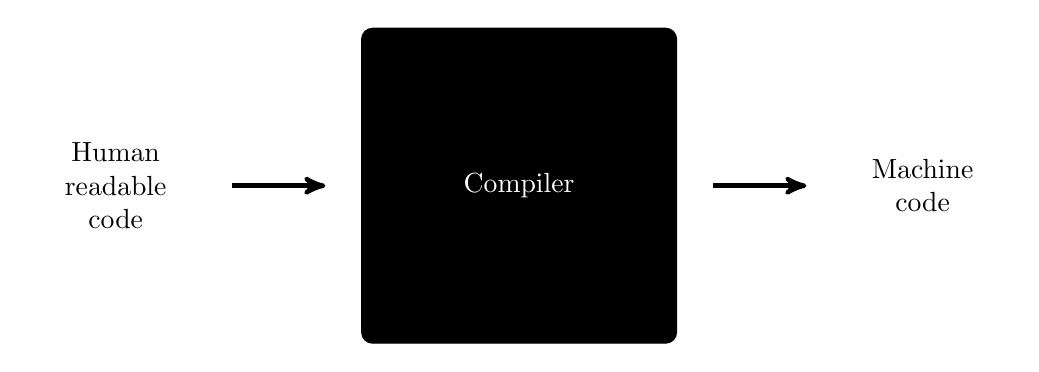
\begin{tikzpicture}
		\node(A){\parbox{2cm}{\centering Human readable code}};
		\coordinate[right=4cm of A](B){};
		\draw[fill=black,rounded corners] ($(B.south west) - (2,2)$) rectangle ($(B.north west) + (2,2)$);
		\node[color=white] (CC) at (B) {Compiler};
		\node[right=4cm of B](C){\parbox{2cm}{\centering Machine code}};
		\draw[->,>=stealth',shorten <=10,shorten >=70,ultra thick] (A) -- (B);
		\draw[->,>=stealth',shorten <=70,shorten >=10,ultra thick] (B) -- (C);
	\end{tikzpicture}
	\end{center}
\end{frame}

\begin{frame}
	\frametitle{Inside your computer}
	\begin{center}
	\begin{tikzpicture}
		\only<1>{\node(A){\includegraphics[width=.5\textwidth]{img/sandy_bridge}};}
		\only<2->{\node(A){\includegraphics[width=.5\textwidth]{img/sandy_bridge_annotated}};}
		\uncover<3->{%
		\node[below=of A](R){\includegraphics[width=.5\textwidth]{img/ram-w}};
		\draw[->,very thick,>=stealth',shorten >=-20] (A) -- (R);
		\draw[->,very thick,>=stealth',shorten <=-20] (R.80) -- (A.280);
		}%
		\uncover<4->{%
		\node[draw,right=1.8cm of A](S){Sound card};
		\node[draw,above=0.8cm of S](G){Graphics card};
		\node[draw,below=0.8cm of S](H){Hard drive};
		\draw[->,very thick,>=stealth',shorten >=10] (A) -- (G.180);
		\draw[->,very thick,>=stealth',shorten >=10] (A) -- (S.180);
		\draw[->,very thick,>=stealth',shorten >=10] (A) -- (H.180);
		}%
	\end{tikzpicture}
	\end{center}
\end{frame}

\begin{frame}
	\frametitle{Inside the CPU}
	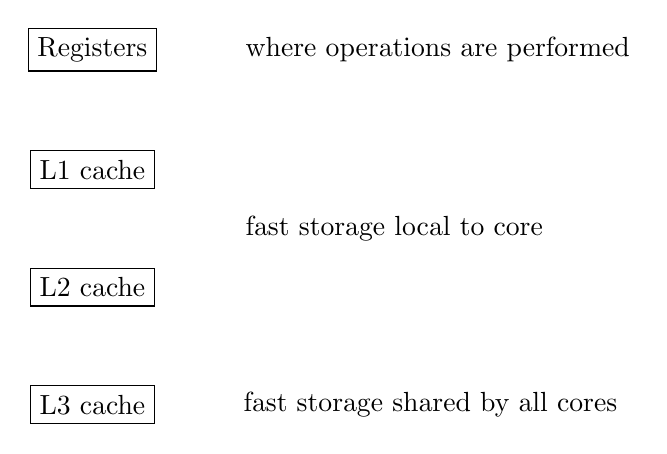
\begin{tikzpicture}
		\node[draw](A){Registers};
		\node[draw,below=of A](B) {L1 cache};
		\node[draw,below=of B](C) {L2 cache};
		\node[draw,below=of C](D) {L3 cache};
		\path(B) -- node[midway](m){} (C);
		\node[right=of A,anchor=west](a) {where operations are performed};
		\node[anchor=west](b) at (m -| a.west) {fast storage local to core};
		\node[right=of D,anchor=west](d) {fast storage shared by all cores};
	\end{tikzpicture}
\end{frame}

\begin{frame}
	\frametitle{Rough assembly introduction}
	\begin{center}
	{\setlength{\tabcolsep}{1.5em}\renewcommand{\arraystretch}{1.5}%
	\begin{tabular}[]{ll}
		\texttt{rxx} & 64 bit register called \texttt{xx} \\
		\texttt{exx} & 32 bit register called \texttt{xx} \\
		\texttt{DWORD PTR [a]} & reference to memory address \texttt{a} \\
		\texttt{j* label} & (conditional) jump to \texttt{label} \\
		\texttt{mov a, b} & copy \texttt{b} into \texttt{a} \\
		\texttt{add a, b} & add the value of \texttt{b} to \texttt{a} \\
	\end{tabular}}
	\end{center}
\end{frame}

\begin{frame}[fragile]
	\frametitle{How can you swap two variables?}
\newsavebox{\swapverb}%
\begin{lrbox}{\swapverb}\begin{minipage}{.6\textwidth}%
\begin{verbatim}
/**
 * Swaps a and b.
 */
void swap( int& a, int& b ) {
  /* ??? */
}
\end{verbatim}
\end{minipage}\end{lrbox}%
	\begin{center}\usebox{\swapverb}\end{center}
\end{frame}

\begin{frame}
	\frametitle{So\ldots whats the point?}
	Use the optimizer: \texttt{-O3 -march=native}

	Don't worry too much --- the compiler will probably change your code anyway.
\end{frame}

\end{document}

